% !TEX TS-program = pdflatex
% !TEX encoding = UTF-8 Unicode

% This file is a template using the "beamer" package to create slides for a talk or presentation
% - Giving a talk on some subject.
% - The talk is between 15min and 45min long.
% - Style is ornate.

% MODIFIED by Jonathan Kew, 2008-07-06
% The header comments and encoding in this file were modified for inclusion with TeXworks.
% The content is otherwise unchanged from the original distributed with the beamer package.

\documentclass{beamer}
\setbeamercovered{invisible}



% Copyright 2004 by Till Tantau <tantau@users.sourceforge.net>.
%
% In principle, this file can be redistributed and/or modified under
% the terms of the GNU Public License, version 2.
%
% However, this file is supposed to be a template to be modified
% for your own needs. For this reason, if you use this file as a
% template and not specifically distribute it as part of a another
% package/program, I grant the extra permission to freely copy and
% modify this file as you see fit and even to delete this copyright
% notice. 


\mode<presentation>
{
  \usetheme{Warsaw}
  % or ...

  % or whatever (possibly just delete it)
}


\usepackage[english]{babel}
% or whatever

\usepackage[utf8]{inputenc}
% or whatever

\usepackage{times}
\usepackage[T1]{fontenc}
% Or whatever. Note that the encoding and the font should match. If T1
% does not look nice, try deleting the line with the fontenc.

%%% MATH RELATED


%%% AMS math stuff
\usepackage{amsmath}
\usepackage{amssymb}
\usepackage{amsthm}
\usepackage{mathrsfs}
\usepackage{enumerate}

%%% Theorem environments
\newtheorem{thm}{Theorem}[subsection]
\newtheorem{prop}[thm]{Proposition}
\newtheorem{cor}{Corollary}[thm]
\newtheorem{por}[thm]{Porism}
\newtheorem{lem}[thm]{Lemma}
\theoremstyle{definition}
\newtheorem{prob}[thm]{Problem}
\newtheorem{soln}{Solution}
\newtheorem{defn}[thm]{Definition}
\newtheorem{ex}[thm]{Example}
\newtheorem{quest}[thm]{Question}
\newtheorem{remk}[thm]{Remark}

%%% Typesetting shortcuts
\newcommand{\tn}[1]{\textnormal{#1}}
\newcommand{\ol}[1]{\overline{#1}}
\newcommand{\wt}[1]{\widetilde{#1}}
\newcommand{\wh}[1]{\widehat{#1}}
\newcommand{\vocab}[1]{\textbf{#1}\index{#1}}

%%% Math shortcuts
\newcommand{\bbr}{\mathbb R}
\newcommand{\bbz}{\mathbb Z}
\newcommand{\bbq}{\mathbb Q}
\newcommand{\bbn}{\mathbb N}
\newcommand{\bbf}{\mathbb F}
\newcommand{\bbc}{\mathbb C}
\newcommand{\bbd}{\mathbb D}
\newcommand{\bba}{\mathbb A}
\newcommand{\bbp}{\mathbb P}
\newcommand{\bbg}{\mathbb G}
\newcommand{\bbv}{\mathbb V}
\newcommand{\dih}[1]{\mathcal D_{#1}}
\newcommand{\sym}[1]{\mathcal S_{#1}}
\newcommand{\vspan}{\tn{span}}
\newcommand{\trace}{\tn{trace}}
\newcommand{\diff}{\backslash}
\newcommand{\stab}{\tn{stab}}
\newcommand{\conv}{\tn{conv}}
\newcommand{\img}{\tn{img}}
\newcommand{\coker}{\tn{coker}}
\newcommand{\id}{\tn{id}}
\newcommand{\Hom}{\tn{Hom}}
\newcommand{\End}{\tn{End}}
\newcommand{\Aut}{\tn{Aut}}
\newcommand{\aut}{\tn{Aut}}
\newcommand{\ann}{\tn{Ann}}
\newcommand{\GL}{\tn{GL}}
\newcommand{\Gr}{\tn{Gr}}
\newcommand{\lord}{\preccurlyeq}
\newcommand{\rord}{\succcurlyeq}
\newcommand{\tr}{\textnormal{Tr}}
\newcommand{\Tr}{\textnormal{Tr}}
\newcommand{\bbl}{\mathbb{L}}
\newcommand{\C}{\mathscr{C}}
\newcommand{\X}{\mathscr{X}}
\renewcommand{\S}{\mathscr{S}}
\newcommand{\M}{\mathscr{M}}
\renewcommand{\L}{\mathcal{L}}


%%% Algebraic Geometry
\newcommand{\height}{\textnormal{ht}}
\newcommand{\A}{\mathbb{A}}
\newcommand{\p}{\mathfrak{p}}
\newcommand{\sheaf}[1]{\mathcal{#1}}
\newcommand{\spec}{\textnormal{Spec}}
\newcommand{\proj}{\textnormal{Proj}}
\newcommand{\Aff}{\textnormal{Aff}}
\newcommand{\skel}{\textnormal{skel}}
\newcommand{\supp}{\textnormal{supp}}
\newcommand{\orb}{\textnormal{orb}}
\newcommand{\Proj}{\textnormal{Proj}}
\newcommand{\Pic}{\textnormal{Pic}}
\newcommand{\Rees}{\textnormal{Rees}}
\newcommand{\shom}{\mathcal{H}om}

\renewcommand*\arraystretch{1.3}

%%% paper specific definitions
\newcommand{\weyl}{\Omega}
\newcommand{\weyll}{{\widehat{\Omega}}}
\newcommand{\weylll}{{\widetilde{\Omega}}}
\newcommand{\mweyl}{{M_N(\Omega)}}
\newcommand{\mweyll}{{M_N(\widehat{\Omega})}}
\newcommand{\mweylll}{{M_N(\widetilde{\Omega})}}
\newcommand{\seq}{\text{Seq}}
\newcommand{\tail}{\text{Tail}}
\newcommand{\Ad}{\textnormal{Ad}}
\newcommand{\sech}{\textnormal{sech}}
\newcommand{\colim}{\varinjlim}
\newcommand{\limit}{\varprojlim}
\newcommand{\Bis}{\textnormal{Bis}}
\newcommand{\m}{\mathfrak{m}}
\newcommand{\mxx}[4]{\left(\begin{array}{cc} #1 & #2\\ #3 & #4 \end{array}\right)}
\newcommand{\diag}{\text{diag}}
\newcommand{\qdet}{\textnormal{qdet}}
\newcommand{\mdet}{\textnormal{mdet}}
\newcommand{\mtau}{\mathcal{T}}
\newcommand{\cof}{\textnormal{cof}}
\newcommand{\minor}{\textnormal{minor}}
\newcommand{\holo}{Holo}
\newcommand{\ord}{\textnormal{order}}
\newcommand{\mult}{\mathfrak M}






\title{MATH 350-2 Advanced Calculus} 
\subtitle
{} % (optional)

\author[W.R. Casper] % (optional, use only with lots of authors)
{W.R. Casper}
% - Use the \inst{?} command only if the authors have different
%   affiliation.

\institute[California State University Fullerton] % (optional, but mostly needed)
{
  Department of Mathematics\\
  California State University Fullerton}
% - Use the \inst command only if there are several affiliations.
% - Keep it simple, no one is interested in your street address.

\subject{Talks}
% This is only inserted into the PDF information catalog. Can be left
% out. 



% If you have a file called "university-logo-filename.xxx", where xxx
% is a graphic format that can be processed by latex or pdflatex,
% resp., then you can add a logo as follows:

% \pgfdeclareimage[height=0.5cm]{university-logo}{university-logo-filename}
% \logo{\pgfuseimage{university-logo}}



% Delete this, if you do not want the table of contents to pop up at
% the beginning of each subsection:
\AtBeginSubsection[]
{
  \begin{frame}<beamer>{Outline}
    \tableofcontents[currentsection,currentsubsection]
  \end{frame}
}


% If you wish to uncover everything in a step-wise fashion, uncomment
% the following command: 

%\beamerdefaultoverlayspecification{<+->}


\begin{document}

\begin{frame}
  \titlepage
\end{frame}

\begin{frame}{Outline}
  \tableofcontents
  % You might wish to add the option [pausesections]
\end{frame}

% Since this a solution template for a generic talk, very little can
% be said about how it should be structured. However, the talk length
% of between 15min and 45min and the theme suggest that you stick to
% the following rules:  

% - Exactly two or three sections (other than the summary).
% - At *most* three subsections per section.
% - Talk about 30s to 2min per frame. So there should be between about
%   15 and 30 frames, all told.

\section{Real Analysis Lecture 1}
\subsection{Origin of Real Numbers}

\begin{frame}{Prehistoric numbers}
  \hfil\hfil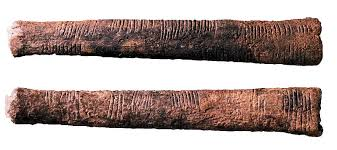
\includegraphics[width=5cm]{fig/ishango}\newline
  \null\hfil\hfil\makebox[5cm]{20,000 BC tallies on Ishango bone}\newline
  \vfil
  \hfil\hfil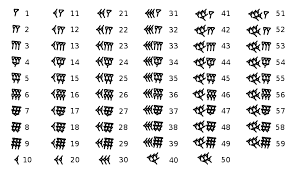
\includegraphics[width=5cm]{fig/sumerian}\hfil\hfil
    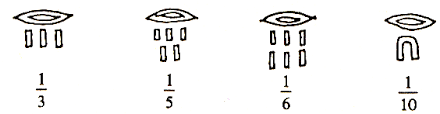
\includegraphics[width=5cm]{fig/egyptian}\vfil
  \null\hfil\hfil\makebox[5cm]{3400 BC Sumerian system}
    \hfil\hfil\makebox[5cm]{1000 BC Egyptian fractions}
\end{frame}

\begin{frame}{Invention of zero}
\begin{itemize}
\pause
\item 1770 BC - concept of zero in heiroglyph
\pause
\item 36 BC - Mayan/Olmec heiroglyph for zero
\pause
\item 150 AD - Ptolemy using it in astronomy
\pause
\item medieval scholars - debating the existence of $0$
\end{itemize}\vfil

\includegraphics[width=\linewidth]{fig/zeros}
\end{frame}

\begin{frame}{Invention of negatives}
\begin{itemize}
\pause
\item 100-50 BC - concept of negatives in China
\pause
\item 628 AD - used in India in quadratic formula
\pause
\item 9th century - Islamic mathematicians invent algebra, but hesitant about negatives
\pause
\item 12th century - Islamic mathematicians add negative solutions of quadratics, but discard them
\pause
\item 1202,1225 - Fibonacci allows negatives as solutions for financial problems
\pause
\item up to 18th century - rejected by western sources, referred to as "absurd numbers"
\end{itemize}
\end{frame}

\begin{frame}{Invention of rationals}
\begin{itemize}
\pause
\item 1000 BC - appear in Egyptian heiroglyphs
\pause
\item Greek and Indian mathematicians used them regularly in studying number theory
\pause
\item 300 BC -appear in Euclid's elements
\end{itemize}\vfil
\begin{center}
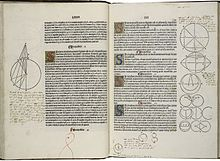
\includegraphics[height=1in]{fig/elements}
\end{center}
\end{frame}

\begin{frame}{Discovery of irrationals}
\begin{itemize}
\pause
\item 800 BC - Indian mathematicians discuss nonrationality of square roots
\pause
\item 500 BC - Greek mathematicians discover the existence of irrational numbers (sides of the pentagram)
\pause
\item discovered by Hippasus, who legend says was thrown into the sea for his discovery
\pause
\item 14th-16th century - Indian mathematicians discover infinite series expressions for $\pi$
\pause
\item 17th century - European mathematicians distinguish between transcendentals and algebraic numbers
\end{itemize}
\end{frame}

\subsection{Properties of real numbers}

\begin{frame}{Philosophy of our presentation}
\begin{itemize}
\pause
\item we will not construct the reals (ref. Foundations of Analysis by Landau for a rigorous construction from the ground up using minimal axioms and Dedekind cuts)
\pause
\item instead, we will take for granted that the reals exist and describe ten fundamental rules (axioms) for how it behaves
\pause
\item the integers, rationals, etc. will be defined in terms of the reals
\end{itemize}
\end{frame}


\begin{frame}{Field axioms}
A \textbf{field} is a set $F$ with a way to do addition $+$ and multiplication $\times$ with
\begin{enumerate}[\text{A}1]
\pause
\item \textbf{commutativity}: $x+y = y+x$ and $xy=yx$
\pause
\item \textbf{associativity}: $(x+y) + z = x + (y+z)$ and $(xy)z = x(yz)$
\pause
\item \textbf{distributivity}: $x(y + z) = xy + xz$
\pause
\item \textbf{additive inverse}: given $x,y\in F$, there exists a unique $z\in F$ with $x=y+z$
$$\text{Notation:}\quad z := x-y$$
\pause
\item \textbf{multiplicative inverse}: given $x,y\in F$ with $y\neq 0$, there exists a unique $z\in F$ with $x = yz$
$$\text{Notation:}\quad z := x/y$$
\end{enumerate}
\pause
\textbf{Special notation:} $0:= x-x$ and $1:= x/x$, and $-x := 0-x$
\end{frame}

\begin{frame}{Challenge!}
\begin{prob}
use the axioms to show that $(x+y)z = xz + yz$.
\end{prob}
\pause
\begin{soln}
$$(x+y)z \stackrel{A1}{=} z(x+y) \stackrel{A3}{=} zx + zy \stackrel{A1}{=} xz + yz.$$
\end{soln}
\end{frame}

\begin{frame}{Challenge!}
\begin{prob}
use the axioms to show that the value of $x-x$ doesn't depend on $x$.
\end{prob}
\pause
\begin{soln}
Suppose $z_1=x-x$ and $z_2=y-y$.\\
\pause
Then $x = x+z_1$ and $y=y+z_2$.\\
\pause
Therefore we have
$$(x+y)+z_1\stackrel{A2}{=}x+(y+z_1)\stackrel{A1}{=}x+(z_1+y)\stackrel{A2}{=}(x+z_1) + y=x+y,$$
\pause
$$(x+y)+z_2\stackrel{A2}{=}x+(y+z_2)=x+y,$$
\pause
so that
$$z_1 = (x+y)-(x+y) = z_2.$$
\end{soln}
\end{frame}

\begin{frame}{Challenge!}
\begin{prob}
use the axioms to show that the value of $x/x$ doesn't depend on $x$.
\end{prob}
\pause
\begin{soln}
Suppose $z_1=x/x$ and $z_2=y/y$.\\
\pause
Then $x = z_1x$ and $y=z_2y$.\\
\pause
Therefore we have
$$z_1(xy) \stackrel{A2}{=} (z_1x)y = xy,$$
\pause
$$z_2(xy) \stackrel{A2}{=} (z_2x)y \stackrel{A1}{=} (xz_2)y \stackrel{A2}{=} x(z_2y) = xy,$$
\pause
so that
$$z_1 = (xy)/(xy) = z_2.$$
\end{soln}
\end{frame}

\begin{frame}{Field examples}
Lots of examples of fields!
\begin{itemize}
\pause
\item \textbf{rational numbers}
$$\mathbb{Q} = \{ a/b: a,b\ \text{integers with}\ b\neq 0\}.$$
\pause
\item \textbf{real numbers} $\mathbb{R}$ (what are they?)
\pause
\item \textbf{complex numbers}
$$\mathbb{C} = \{ a + ib: a,b\ \text{real numbers}\}.$$
\pause
\item \textbf{field of Boolean numbers}
$$\mathbb{F}_2 = \{0,1\}$$
$$0+0 = 0,\quad 0+1 = 1,\quad 1+0 = 1,\quad 1+1 = 0$$
$$0\cdot 0 = 0,\quad 0\cdot1 = 0,\quad 1\cdot0 = 0,\quad 1\cdot1 = 1$$
\end{itemize}
\end{frame}

\begin{frame}{Challenge!}
\begin{prob}
explain why the set of integers isn't a field
\end{prob}
\pause
\begin{soln}
There aren't multiplicative inverses!
\pause
For example, $1/2$ doesn't make sense because there isn't an integer $z$ with $1=2z$.
\end{soln}
\end{frame}

\begin{frame}{Order axioms}
An \textbf{ordered field} is a field $F$ with a relation $<$ 
\begin{enumerate}[\text{A}1]
\setcounter{enumi}{5}
\pause
\item \textbf{trichotomy}: for any $x,y\in F$, exactly one of the following holds:
$$x < y,\quad y < x,\quad\text{or}\quad x = y$$
\pause
\item \textbf{compatible with $+$}: $x < y$ implies $x+z < y+z$
\pause
\item \textbf{compatible with $\times$}: $0 < x$ and $0 < y$ implies $0 < xy$
\pause
\item \textbf{transitivity}: $x < y$ and $y < z$ implies $x < z$
\end{enumerate}
\pause
\textbf{Special notation:}
\begin{itemize}
\item $x > y$ means $y < x$
\item $x \leq y$ means $x < y$ or $x=y$
\item $x \geq y$ means $y \leq x$
\end{itemize}
\end{frame}

\begin{frame}{Challenge!}
\begin{prob}
explain why $\mathbb{F}_2$ cannot be made into an ordered field
\end{prob}
\pause
\begin{soln}
There is no way to put an order relation $<$ on it!\\
\pause
The trichotomy (Axiom 6) would say either $0 < 1$ or $1 < 0$.\\
\pause
If $0 < 1$, then by Axiom 7
$$ 1 = 0+1 < 1+1 = 0$$
but this means both $0 < 1$ and $1 < 0$, which violates the trichotomy.
\pause
Same outcome if $1 < 0$.
\end{soln}
\end{frame}

\begin{frame}{Apostol Theorem 1.1}
\begin{thm}
If $a < b + \epsilon$ for all $\epsilon > 0$, then $a\leq b$.
\end{thm}
\pause
\begin{proof}
(Contradiction.)  Assume the statement is false.\\
\pause
Then the trichotomy says $a > b$.\\
\pause
This means $a-b > 0$ by A7.\\
\pause
This means $(a-b)/2 > 0$ by A8.\\
\pause
This means
$$a < b + \frac{a-b}{2} = \frac{a+b}{2} \stackrel{\text{A7\&A8}}{<} \frac{a+a}{2} = a.$$
\pause
This says $a < a$, which contradicts the trichotomy.
\end{proof}
\end{frame}

\end{document}


